\section{Results}
\label{sec:Results}
In this section, we present the results obtained by running \ApproachName{} and the SBPCG benchmark on \CaseStudy{}.
Table~\ref{tab:resultsMeanStDevRQ12} shows the mean values and standard deviations for $Q_{Duration}$ for each \ApproachName{} variant and the SBPCG benchmark, while Figure~\ref{fig:results} shows the results in form of boxplots, grouped per host (i.e., the boss of \CaseStudy{} used in our experiment, namely Argos, Maia, Orion, Teuthus, and Vermis) and overall.  Each boxplot represnts the distribution of $Q_duration$ values (obtained as average of 30 independent runs) for each of the 645 solutions obtained from transplantation \ApproachName{} (\simhotep{} and \timhotep{}) and SBPCG.
%. Each boxplot represents 645 values of a specific host-organ transplantation (\ApproachName{}) or 645 generations from a specific host (Baseline). Each value in the boxplot is the mean value (between the 30 independent runs) of the quality indicator ($Q_{Duration}$) for one of the transplants (\ApproachName{}) or generations (Baseline). 

We can observe that both variants (\simhotep{} and \timhotep{}) obtained better results than the SBPCG benchmark. Specifically, \simhotep{} yielded the best results, followed by \timhotep{} and then SBPCG. The variants obtained an average value of 44.85\% in $Q_{Duration}$, with \simhotep{} being the variant that obtained the best results overall (53.31\% in $Q_{Duration}$). \timhotep obtained 36.39\% in the overall $Q_{Duration}$, which also outperformed SBPCG. SBPCG obtained the worst $Q_{Duration}$. Overall, the results reveal that leveraging simulations as objective function pays off in the context of PCT, yielding 1.5x better results than the \timhotep{} and 2.5x better results than the SBPCG benchmark.

% \begin{table*}[tb]
% \centering
% \caption{RQ1-RQ2. Mean values and standard deviations for $Q_{Duration}$ for each approach per Host and Overall.}
% \label{tab:resultsMeanStDevRQ12}
% \resizebox{.65\textwidth}{!}{
% \begin{tabular}{@{}lrrrrrr@{}}
% \toprule
% & Argos            & Maia              & Orion            & Teuthus           & Vermis            & Overall           \\ \midrule
% \rowcolor[HTML]{C0C0C0}
% \multicolumn{1}{r}{\cellcolor[HTML]{FFFFFF}{$S_{Imhotep}$}} 
% & 43.92 $\pm$ 9.30 & 43.08 $\pm$ 12.09 & 48.86 $\pm$ 8.69 & 60.78 $\pm$ 7.38  & 69.90 $\pm$ 10.52 & 53.31 $\pm$ 14.26 \\ \midrule
% \multicolumn{1}{r}{$T_{Imhotep}$} & 32.17 $\pm$ 6.94 & 29.52 $\pm$ 9.34  & 31.41 $\pm$ 6.83 & 46.33 $\pm$ 10.54 & 42.50 $\pm$ 12.96 & 36.39 $\pm$ 11.72 \\ \midrule
% \multicolumn{1}{r}{Baseline} & 20.15 $\pm$ 1.86 & 8.43 $\pm$ 1.81   & 32.97 $\pm$ 0.85 & 19.53 $\pm$ 1.88  & 25.48 $\pm$ 3.31  & 21.31 $\pm$ 8.32  \\ \bottomrule
% \end{tabular}
% }
% \end{table*}

When analysing whether there is statistical significant differences among the results obtained by \simhotep{} and Base. We found that the obtained $p-values$ for $Q_{Duration}$ are always lower than $4.01x10^{-23}$  (see Table \ref{tab:resultsWilcEffRQ1}). This is below the significance threshold value, so we can comfortably state that \simhotep{} provides significant better values for $Q_{Duration}$ with respect to Base. We also observe that all the  A12 effect size values are large (see Table \ref{tab:resultsWilcEffRQ1}), thus confirming the practical magnitude of such a difference. Thus, we conclude that:

\noindent \textbf{Answer to RQ$_1$} \simhotep{} performance far surpasses the baseline with statistically significant results and large effect size in all cases, and exhibiting a remarkable overall enhancement of 250\% over SBPCG.

\begin{table}[tb]	
\caption{(a) RQ1-RQ2. Mean values and standard deviations for $Q_{Duration}$ for each approach per Host and Overall. (b) Mann-Withney U pair-wise test results / Vargha-Delaney Â$_{12}$ effect sizes obtained comparing \simhotep{} Vs. Base (RQ1) and \simhotep{} Vs. \timhotep{} (RQ2) per host and overall. Â$_{12}$: Large -- L.}
	\label{tab:resultsRQ12}
\begin{subtable}{.5\columnwidth}
    \caption{Mean values and standard deviations.}
    \label{tab:resultsMeanStDevRQ12}
    \centering
    \resizebox{\columnwidth}{!}{
	\begin{tabular}{@{}lccc@{}}
		\toprule  & \simhotep{} & \timhotep{} & Base        \\ \cmidrule(l){2-4} 
		Boss & Mean $\pm$ StDev & Mean $\pm$ StDe & Mean $\pm$ StDe  \\ \midrule 
		Argos  & 43.92 $\pm$ 9.30  & 32.17 $\pm$ 6.94 & 20.15 $\pm$ 1.86 \\
		Maia  & 43.08 $\pm$ 12.09  & 29.52 $\pm$ 9.34 & 8.43 $\pm$ 1.81   \\
		Orion  & 48.86 $\pm$ 8.69 & 31.41 $\pm$ 6.83 & 32.97 $\pm$ 0.85 \\
		Teuthus & 60.78 $\pm$ 7.38  & 46.33 $\pm$ 10.54 & 19.53 $\pm$ 1.88  \\
		Vermis   & 69.90 $\pm$ 10.52 & 42.50 $\pm$ 12.96 & 25.48 $\pm$ 3.31  \\
        \rowcolor[HTML]{F3F3F3}
		Overall & 53.31 $\pm$ 14.26 & 36.39 $\pm$ 11.72 & 21.31 $\pm$ 8.32   \\
		\bottomrule
	\end{tabular}}
\end{subtable}
\begin{subtable}{.48\columnwidth}
    \caption{Mann-Withney U pair-wise / Vargha-Delaney Â$_{12}$.}
 	\label{tab:resultsWilcEffRQ1}
    \centering
    \resizebox{\columnwidth}{!}{
	\begin{tabular}{@{}lcc@{}}
		\toprule
        & RQ1 & RQ2  \\ \cmidrule(l){2-3} 
		Boss    & $p-Value$ / Â$_{12}$    & $p-Value$ / Â$_{12}$\\ \midrule 
		Argos   & $3.25x10^{-23}$  / 0.99 (L)  & $1.28x10^{-18}$ / 0.85 (L) \\
		Maia    & $3.25x10^{-23}$  /  1.0 (L)  & $6.64x10^{-18}$ / 0.85 (L)  \\
		Orion   & $4.01x10^{-23}$  / 0.98 (L)  & $4.95x10^{-22}$ / 0.95 (L)\\
		Teuthus & $3.25x10^{-23}$  /  1.0 (L)  & $3.60x10^{-18}$ / 0.87 (L)  \\
		Vermis  & $3.25x10^{-23}$  /  1.0 (L)  & $8.86x10^{-23}$ / 0.95 (L)  \\
        \rowcolor[HTML]{F3F3F3}
		Overall & $1.41x10^{-107}$ / 0.98 (L)  & $6.58x10^{-93}$ / 0.82 (L) \\
		\bottomrule
	\end{tabular}}
\end{subtable}
\end{table}

% \begin{table}[tb]
% 	\centering
% 	\caption{RQ1. Mann-Withney U pair-wise test results / Vargha-Delaney Â$_{12}$ effect sizes obtained comparing \simhotep{} Vs. Base per host and overall. Â$_{12}$: Large -- L.}
% 	\label{tab:resultsWilcEffRQ1}
% 	\resizebox{\columnwidth}{!}{
% 	\begin{tabular}{@{}lccccc@{}}
% 		\toprule
%         & RQ1 & RQ2   & \simhotep{} & \timhotep{} & Base        \\ \cmidrule(l){2-6} 
% 		Boss    & $p-Value$ / Â$_{12}$    & $p-Value$ / Â$_{12}$  & Mean $\pm$ StDev & Mean $\pm$ StDe & Mean $\pm$ StDe  \\ \midrule 
% 		Argos   & $3.25x10^{-23}$  / 0.99 (L)  & $1.28x10^{-18}$ / 0.85 (L) & 43.92 $\pm$ 9.30  & 32.17 $\pm$ 6.94 & 20.15 $\pm$ 1.86 \\
% 		Maia    & $3.25x10^{-23}$  /  1.0 (L)  & $6.64x10^{-18}$ / 0.85 (L) & 43.08 $\pm$ 12.09  & 29.52 $\pm$ 9.34 & 8.43 $\pm$ 1.81   \\
% 		Orion   & $4.01x10^{-23}$  / 0.98 (L)  & $4.95x10^{-22}$ / 0.95 (L)  & 48.86 $\pm$ 8.69 & 31.41 $\pm$ 6.83 & 32.97 $\pm$ 0.85 \\
% 		Teuthus & $3.25x10^{-23}$  /  1.0 (L)  & $3.60x10^{-18}$ / 0.87 (L) & 60.78 $\pm$ 7.38  & 46.33 $\pm$ 10.54 & 19.53 $\pm$ 1.88  \\
% 		Vermis  & $3.25x10^{-23}$  /  1.0 (L)  & $8.86x10^{-23}$ / 0.95 (L)  & 69.90 $\pm$ 10.52 & 42.50 $\pm$ 12.96 & 25.48 $\pm$ 3.31  \\
% 		Overall & $1.41x10^{-107}$ / 0.98 (L)  & $6.58x10^{-93}$ / 0.82 (L)  & 53.31 $\pm$ 14.26 & 36.39 $\pm$ 11.72 & 21.31 $\pm$ 8.32   \\
% 		\bottomrule
% 	\end{tabular}
% }
% \end{table}

% \begin{table}[tb]
% 	\centering
% 	\caption{RQ1. Mann-Withney U pair-wise test results / Vargha-Delaney Â$_{12}$ effect sizes obtained comparing \simhotep{} Vs. Base per host and overall. Â$_{12}$: Large -- L.}
% 	\label{tab:resultsWilcEffRQ1}
% 	\resizebox{.5\columnwidth}{!}{
% 	\begin{tabular}{@{}lrr@{}}
% 		\toprule
%         & RQ1 & RQ2          \\ \cmidrule(l){2-3} 
% 		Boss    & $p-Value$ / Â$_{12}$    & $p-Value$ / Â$_{12}$        \\ \midrule 
% 		Argos   & $3.25x10^{-23}$  / 0.99 (L)  & $1.28x10^{-18}$ / 0.85 (L)   \\
% 		Maia    & $3.25x10^{-23}$  /  1.0 (L)  & $6.64x10^{-18}$ / 0.85 (L)   \\
% 		Orion   & $4.01x10^{-23}$  / 0.98 (L)  & $4.95x10^{-22}$ / 0.95 (L)   \\
% 		Teuthus & $3.25x10^{-23}$  /  1.0 (L)  & $3.60x10^{-18}$ / 0.87 (L)   \\
% 		Vermis  & $3.25x10^{-23}$  /  1.0 (L)  & $8.86x10^{-23}$ / 0.95 (L)    \\
% 		Overall & $1.41x10^{-107}$ / 0.98 (L)  & $6.58x10^{-93}$ / 0.82 (L)    \\
% 		\bottomrule
% 	\end{tabular}
% }
% \end{table}

% \begin{table}[tb]
%     \centering
%     \caption{RQ2. Mann-Withney U pair-wise test results / Vargha-Delaney Â$_{12}$ effect sizes obtained comparing \simhotep{} Vs. \timhotep{} per host and overall. Â$_{12}$: Large -- L.}
% 	\label{tab:resultsWilcEffRQ2}
% 	\resizebox{.4\columnwidth}{!}{
%     \begin{tabular}{@{}lr@{}}
%     \toprule
%     Boss    & $p-Value$ / Â$_{12}$           \\ \midrule 
%     Argos   & $1.28x10^{-18}$ / 0.85 (L)     \\
%     Maia    & $6.64x10^{-18}$ / 0.85 (L)     \\
%     Orion   & $4.95x10^{-22}$ / 0.95 (L)     \\
%     Teuthus & $3.60x10^{-18}$ / 0.87 (L)     \\
%     Vermis  & $8.86x10^{-23}$ / 0.95 (L)     \\
%     Overall & $6.58x10^{-93}$ / 0.82 (L)     \\
%     \bottomrule
%     \end{tabular}
% }
%     \end{table}
    
As for the comparison between \simhotep{} and \timhotep{} (RQ2),  we observe that all the $p-values$ achieved when comparing the $Q_{Duration}$ distributions provided by the two \ApproachName{} variants are smaller than the significance threshold, thus indicating that the difference in solution quality is statistically significant in favour of \simhotep{}, and always with a large A12 effect size (see Table \ref{tab:resultsWilcEffRQ1}). Therefore, we conclude that:

\noindent  \textbf{Answer to RQ$_2$} \simhotep{} provides significantly better results than \timhotep{} in the context of automated content generation through transplantation, with a large effect size in all cases examined. The efficacy of \simhotep{} demonstrates a 150\% enhancement overall compared to the outcomes of \timhotep{}.

\begin{figure*}[tb]
    \centering
    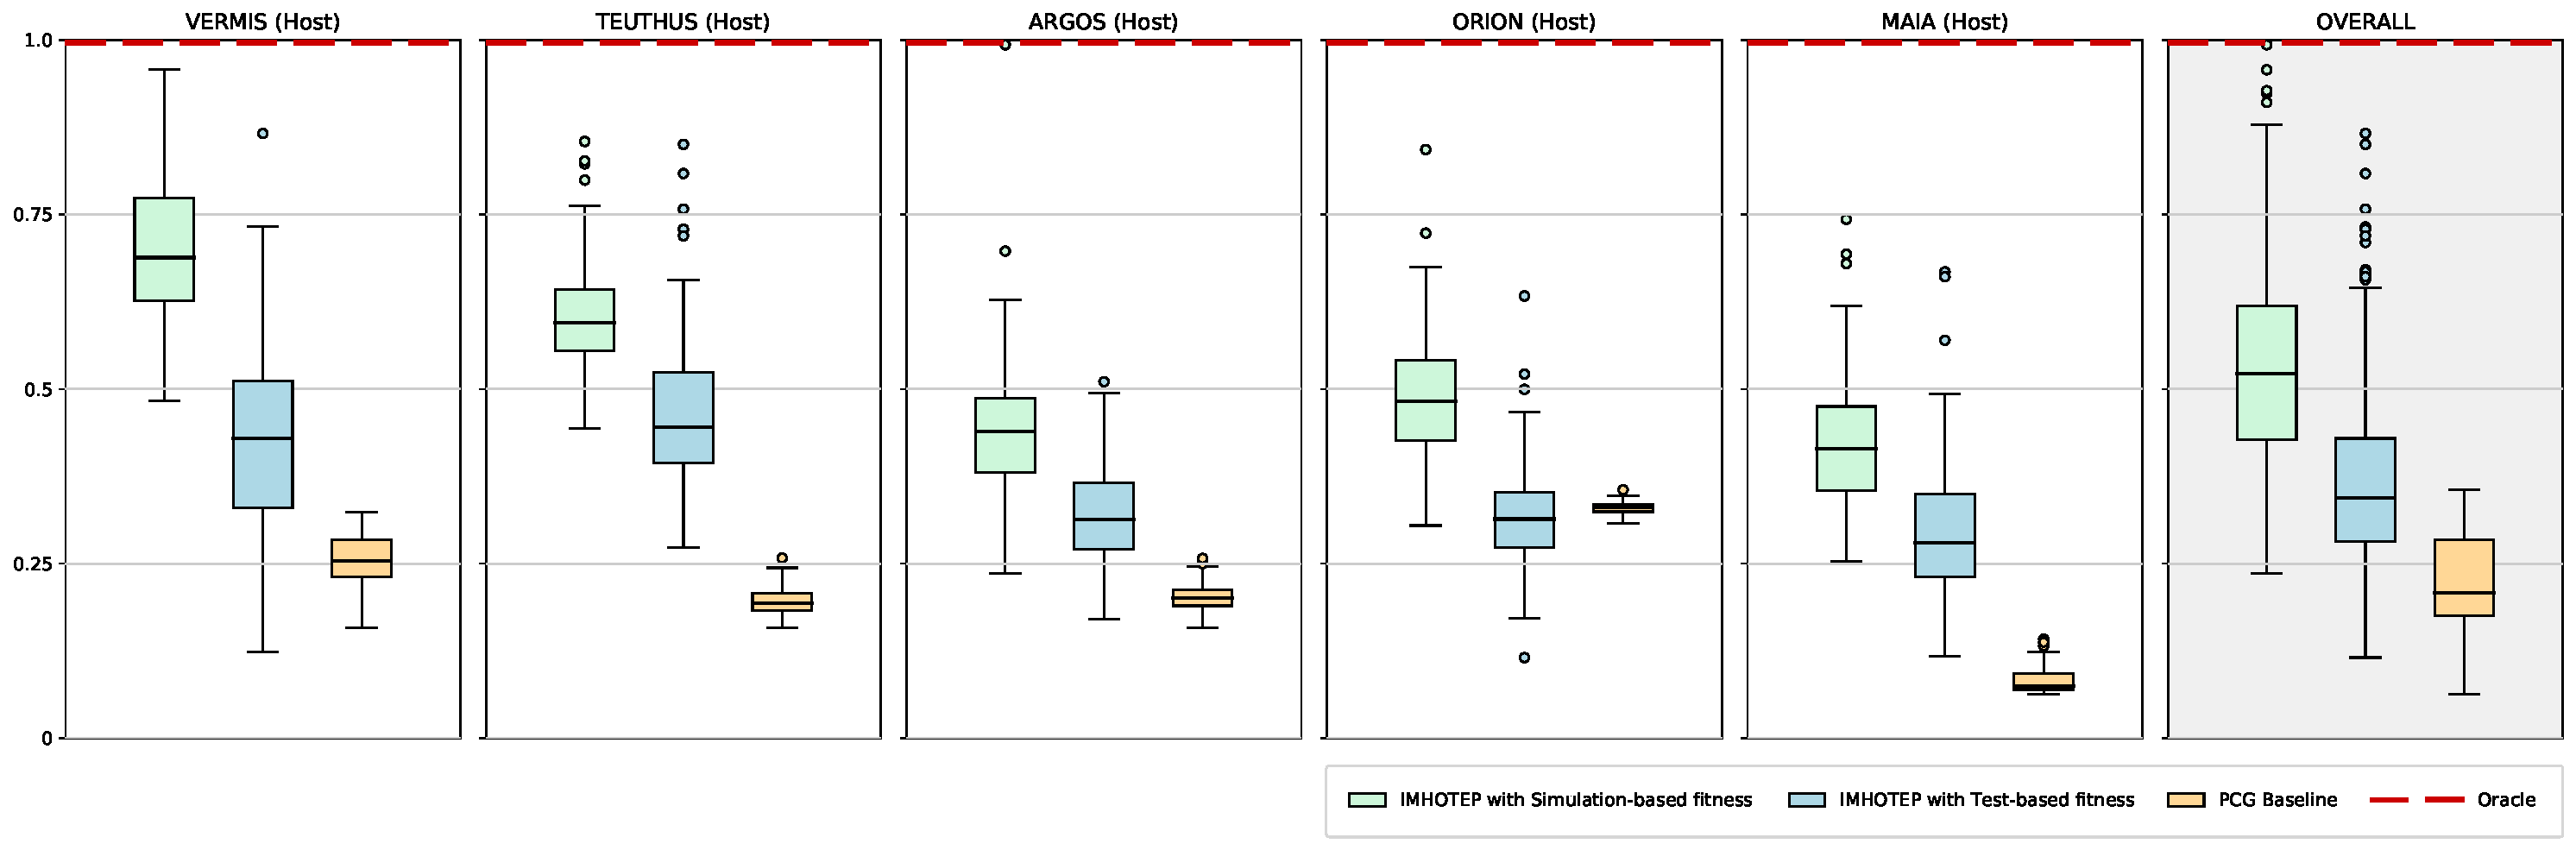
\includegraphics[width=0.8\textwidth]{Figures/Imhotep_with_legend_and_oracle_average-v4.pdf}
    \caption{Results of our \ApproachName{} (\simhotep{} and \timhotep{}) and the SBPCT baseline for the quality measurement ($Q_{Duration}$).}
    \label{fig:results}
\end{figure*}